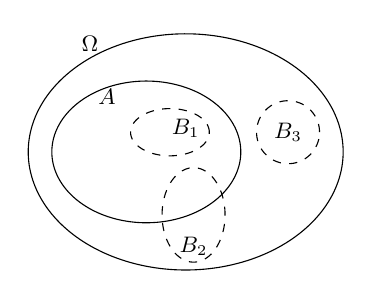
\begin{tikzpicture}%[scale=.9]
\shorthandoff{>}
%
\begin{scope}
%
% Omega, A, B_i
\draw[domain=0:360,samples=200] plot ({2*cos(\x)+.5},{1.5*sin(\x)});
\draw[domain=0:360,samples=200] plot ({1.2*cos(\x)},{.9*sin(\x)});
\draw[dashed,domain=0:360,samples=200] plot ({.5*cos(\x)+.3},{.3*sin(\x)+.25});
\draw[dashed,domain=0:360,samples=200] plot ({.4*cos(\x)+.6},{.6*sin(\x)-.8});
\draw[dashed,domain=0:360,samples=200] plot ({.4*cos(\x)+1.8},{.4*sin(\x)+.25});
%
%
% Omega y A_i's
\draw(-.5,1.375) node[left,scale=.9]{\small $\Omega$};
\draw(-.5,.7) node[scale=.9]{\small $A$};
\draw(.5,.3) node[scale=.9]{\small $B_1$};
\draw(.6,-1.2) node[scale=.9]{\small $B_2$};
\draw(1.8,.25) node[scale=.9]{\small $B_3$};
%
\end{scope}
%
\end{tikzpicture}